% beamer packages
\documentclass{beamer}[12pt]
\usetheme{boxes}
\usecolortheme{seahorse}
\beamertemplatenavigationsymbolsempty
\setbeamertemplate{footline}[frame number]
\setbeamertemplate{items}[triangle]

\setbeamertemplate{enumerate items}{arguments}

%\usepackage{enumitem}


\renewcommand*\footnoterule{}
\newcommand\blfootnote[1]{%
	\begingroup
	\renewcommand\thefootnote{}\footnote{#1}%
	\addtocounter{footnote}{-1}%
	\endgroup
}

% graphics
\usepackage{tikz}
\usepackage{tkz-graph}
\usepackage{pgfplots}
\usepackage{xcolor}

\usepackage{graphicx}
\usepackage{csvsimple}
\usepackage{filecontents}


% pseudocode
\usepackage{algorithmicx}
\usepackage[noend]{algpseudocode}

% maths
\usepackage{amsmath}
\usepackage{amsthm}

\newenvironment{claim}[1]{\par\noindent\underline{Claim:}\newline#1}{}
\renewenvironment{proof}[1]{\par\noindent\underline{Proof:}\newline#1}{}
\renewcommand{\qedsymbol}{}


\begin{document}
	\title{Presentation 4}
	\author{Fynn Lohren, Carsten Schubert, Leon Suchy}
	\date{\today}
	\frame{\titlepage}
	
	\begin{frame}
		\frametitle{Structure}
		\begin{itemize}
			\item Partial MAX-SAT
			\item ILP
			\item Solver Comparison
			\item Heuristic
		\end{itemize}
	\end{frame}


	\begin{frame}
	\frametitle{Partial MAX-SAT}
	\begin{itemize}
		\item Variant of SAT in which a maximum number of clauses shall be satisfied\\
			$\rightarrow$ Hard clauses have to be satisfied \\
			$\rightarrow$ Soft clauses may be satisfied \\
		\pause
		\item MAX-SAT Evaluation taking place annually
		\item Open-WBO one of contending free solvers
		\end{itemize}
	\end{frame}

	\begin{frame}
	\frametitle{Vertex Cover in Partial MAX-SAT}
		Introduce variable $ x_i $ for each vertex $ v_i \in V$ 
		\begin{align*}
			\bigwedge\limits_{\{v_j, v_k\} \in E} & (x_j \lor x_k) \hspace{4mm}\land \tag{Hard clauses}\\
			\bigwedge\limits_{\{v_i\} \in V} & (\neg x_i) \tag{Soft clauses}\\
		\end{align*}
		\pause\
		\qquad $\rightarrow$ Linear in input size
		\vspace*{1.5mm}
		\begin{itemize}
			\item Hard clauses ensure solution is vertex cover
			\item Soft clauses ensure the vertex cover is minimal
		\end{itemize}
	\end{frame}
	
%	\begin{frame}
%		\frametitle{Data Structures}
%		\begin{itemize}[label={-}]
%			\item Heaps
%			\item Bipartite Graph
%			\item Controller
%		\end{itemize}
%	\end{frame}
%	
%	\begin{frame}
%		\frametitle{Bipartite Graph}
%		\begin{columns}[c]
%			\column{.8\textwidth}
%			\hspace{4mm}
%			\begin{tabular}{|l|l|l|l|}\hline
%				Index & Vertex ID & ID left & ID right \\ \hline \hline
%				0 & 0 & 0 & \\ \hline
%				1 & uint\_max - 1 & & 0 \\ \hline
%				2 & 1 & 1 & \\ \hline
%				3 & uint\_max - 2 & & 1 \\ \hline
%				4 & 2 & 2 & \\ \hline
%				5 & NULL & & - \\ \hline
%			\end{tabular}
%			\column{.6\textwidth}
%			
%			\begin{tikzpicture}
%			%\draw[help lines] (0,0) grid (4,4);
%			\SetVertexNormal[
%			Shape 		= circle,
%			LineWidth 	= 1.5pt]
%			\SetUpEdge[
%			lw 		= 1.5pt,
%			color 	= black]
%			
%			\renewcommand{\VertexLightFillColor}{cyan}
%			
%			\Vertex[x=0,y=3,L=$0$]{0}
%			\Vertex[x=0,y=1.5,L=$1$]{2}	
%			\Vertex[x=0,y=0,L=$2$]{4}
%			
%			\renewcommand{\VertexLightFillColor}{red}
%			\Vertex[x=3,y=3,L=$0$]{1}
%			\Vertex[x=3,y=1.5,L=$1$]{3}
%			
%			\Edges(0,1)
%			\Edges(0,3)
%			\Edges(4,3)
%			\end{tikzpicture}
%		\end{columns}
%	\end{frame}
%
%	\begin{frame}
%	\frametitle{Controller}
%	\begin{itemize}[label={-}]
%		\item Too much complexity synchronising all data structures
%		\item Model/View/Controller pattern
%	\end{itemize}
%\end{frame}
%
%	\begin{frame}
%		\frametitle{Clique Cover LB Algorithm}
%		\begin{algorithmic}[1]
%			\Procedure{Clique Cover}{$G(V, E)$}
%			\State $clique\_set \gets \{\}$
%			\State $V \gets sort\_by\_degree(V)$ \Comment{Sort ascending}
%			
%			\ForAll {$v \in V$}
%				\State $clique \gets largest\_clique(v)$ 
%				\Comment{Largest clique v fits in}
%				\State $clique\_set \gets clique\_set \setminus clique$
%				\State $clique \gets clique \cup \{v\}$			
%				\State $clique\_set \gets clique\_set \cup clique$	
%			\EndFor
%			\State 
%			\Return $clique\_set$
%			\EndProcedure
%		\end{algorithmic}
%		
%		\vspace{3mm}
%		Sorting can be computed in $\mathcal{O}(n \log{} n)$ time \\
%		\pause
%		Finding the largest clique for each v can be done in $\mathcal{O}(deg(v))$ time \\
%		\pause
%		More realistic in $\mathcal{O}(\log{} n)$ time\\
%		\pause
%		\text{Total running time: }\\
%		$\mathcal{O}(n \log{} n)$
%	\end{frame}
%	
	
	\begin{frame}
		\frametitle{Open-WBO PMAX-SAT with and without reductions}
			\begin{center}
				Amount of instances solved: \\ \vspace{4mm}
				\begin{tabular}{| l | l | l | l |}
					\hline
					& random & dimacs & snap \\ \hline
					with reductions & 152 & 13 & 7 \\ \hline
					no reductions & 152 & 13 & 2 \\ \hline
				\end{tabular}
			\end{center}
	\end{frame}
	
	\begin{frame}
		\frametitle{Open-WBO PMAX-SAT with and without reductions}
		\begin{tikzpicture}[scale=1]
		\begin{loglogaxis}[
		width=0.9\textwidth,
		height=0.5\textwidth,
		xlabel={{time in s with reductions}\footnote{reductions tested: degree 1, triangle reduction, dominate reduction}},             
		ylabel={{time in s without reductions}},
		legend cell align=left,
		legend pos=north west,
		legend entries={dimacs, random, snap},
		xmax=301,
		xmin=0.01,
		ymax=301,
		ymin=0.01,
		ymode=log,
		] %, meta expr=lg10(\thisrow{vertices}
		\addplot[only marks,color=black, mark=triangle*] table[col sep=comma,y={reds_time}, x={no_reds_time}] {open_wbo_dimacs.csv};
		\addplot[only marks,color=blue, mark=+] table[col sep=comma,y={reds_time}, x={no_reds_time}] {open_wbo_random.csv};
		\addplot[only marks,color=red, mark=square*] table[col sep=comma,y={reds_time}, x={no_reds_time}] {open_wbo_snap.csv};
		\addplot[color=black,domain=0.001:301,samples=4] {x};
		\addplot[dashed,color=black!75,domain=0.01:301,samples=4] {5*x};
		\addplot[dashed,color=black!75,domain=0.01:301,samples=4] {0.2*x};
		\addplot[dotted,color=black,domain=0.01:301,samples=4] {25*x};
		\addplot[dotted,color=black,domain=0.01:301,samples=4] {0.04*x};
		\end{loglogaxis}
		\end{tikzpicture}
	\end{frame}
	
	
	\begin{frame}
	\frametitle{ILP with CPLEX}
	\begin{itemize}
		\item Solve MVC via reduction to ILP.
		\item Used CPLEX
	\end{itemize}
	\end{frame}
	
	\begin{frame}
	\frametitle{CPLEX ILP with and without reductions}
	\begin{center}
		Amount of instances solved: \\ \vspace{4mm}
		\begin{tabular}{| l | l | l | l |}
			\hline
			& random & dimacs & snap \\ \hline
			with reductions & 152 & 22 & 27 \\ \hline
			no reductions & 152 & 22 & 27 \\ \hline
		\end{tabular}
	\end{center}
	\end{frame}


	\begin{frame}
		\frametitle{CPLEX ILP with and without reductions}
		\begin{tikzpicture}[scale=1]
			\begin{loglogaxis}[
			width=0.9\textwidth,
			height=0.5\textwidth,
			xlabel={{time in s, reductions}\footnote{reductions tested: degree 1, triangle reduction, dominate reduction}},             
			ylabel={{time in s, no reductions}},
			legend cell align=left,
			legend pos=north west,
			legend entries={dimacs, random, snap},
			xmax=301,
			xmin=0.01,
			ymax=301,
			ymin=0.01,
			ymode=log,
			] %, meta expr=lg10(\thisrow{vertices}
			\addplot[only marks,color=black, mark=triangle*] table[col sep=comma,y={reds_time}, x={no_reds_time}] {ilp_dimacs.csv};
			\addplot[only marks,color=blue, mark=+] table[col sep=comma,y={reds_time}, x={no_reds_time}] {ilp_random.csv};
			\addplot[only marks,color=red, mark=square*] table[col sep=comma,y={reds_time}, x={no_reds_time}] {ilp_snap.csv};
			\addplot[color=black,domain=0.001:301,samples=4] {x};
			\addplot[dashed,color=black!75,domain=0.01:301,samples=4] {5*x};
			\addplot[dashed,color=black!75,domain=0.01:301,samples=4] {0.2*x};
			\addplot[dotted,color=black,domain=0.01:301,samples=4] {25*x};
			\addplot[dotted,color=black,domain=0.01:301,samples=4] {0.04*x};
			\end{loglogaxis}
		\end{tikzpicture}
	\end{frame}

	\begin{frame}
		\frametitle{ILP Conclusion}
		\begin{itemize}
			\item Data reductions have nearly no impact
			\item Dense graphs are less parallelizable 
			\item Data reductions don't change that
			\item Beware: ILP solution can have float error
		\end{itemize}
	\end{frame}
	
	\begin{frame}
		
	\frametitle{Solver Comparison}
	\begin{figure}
		\begin{tikzpicture}
		\begin{axis}[
		width=0.8\textwidth,
		height=0.6\textwidth,
		grid,
		xlabel={$k$},
		ylabel={$time\ in\ s$},
		xmax=200000,
		xmode=log,
		legend pos=north west]
		
		% \thisrowno needs to be used because it does not find the time key for some reason
		\addplot[only marks, color=blue, mark=*] table[x={Solution VC}, y={Execution Time}, scatter src=\thisrowno{1}, col sep=comma]{ilp_deg0_deg1_triangle_dominate_random.csv};
		\addlegendentry{ILP}
		
		\addplot[only marks, color=blue, mark=+, forget plot] table[x={Solution VC}, y={Execution Time}, scatter src=\thisrowno{1}, col sep=comma]{ilp_deg0_deg1_triangle_dominate_dimacs.csv};
		
		\addplot[only marks, color=blue, mark=triangle*, forget plot] table[x={Solution VC}, y={Execution Time}, scatter src=\thisrowno{1}, col sep=comma]{ilp_deg0_deg1_triangle_dominate_snap.csv};
		
		\addplot[only marks, color=red, mark=*] table[x={Solution VC}, y={Execution Time}, scatter src=\thisrowno{1}, col sep=comma]{open_wbo_deg1_triangle_dominate_random.csv};
		\addlegendentry{SAT}
		
		\addplot[only marks, color=red, mark=+, forget plot] table[x={Solution VC}, y={Execution Time}, scatter src=\thisrowno{1}, col sep=comma]{open_wbo_deg1_triangle_dominate_dimacs.csv};
		
		\addplot[only marks, color=red, mark=triangle*, forget plot] table[x={Solution VC}, y={Execution Time}, scatter src=\thisrowno{1}, col sep=comma]{open_wbo_deg1_triangle_dominate_snap.csv};
		
		\addplot[only marks, color=black, mark=*] table[x={Solution VC}, y={Execution Time}, scatter src=\thisrowno{1}, col sep=comma]{FINALPLUS_0_and_1_and_2_k_dominate_random.csv};
		\addlegendentry{MVC}
		
		\addplot[only marks, color=black, mark=+, forget plot] table[x={Solution VC}, y={Execution Time}, scatter src=\thisrowno{1}, col sep=comma]{FINALPLUS_0_and_1_and_2_k_dominate_dimacs.csv};
		
		\addplot[only marks, color=black, mark=triangle*, forget plot] table[x={Solution VC}, y={Execution Time}, scatter src=\thisrowno{1}, col sep=comma]{FINALPLUS_0_and_1_and_2_k_dominate_snap.csv};
		\end{axis}
		\end{tikzpicture}
	\end{figure}
\end{frame}
	
	\begin{filecontents*}{feocean.csv}
		degree,vertices
		1,38
		2,456
		3,2656
		4,6217
		5,19020
		6,115050
	\end{filecontents*}
	
	\begin{frame}
	\frametitle{Heuristic Tricks}
	\begin{itemize}
		\item apply degree 1, 2 and dominate reduction
		\item choose vertex with max degree
		\item after deleting look at neighbours
		\item search for paths starting from neighbours
	\end{itemize}
\end{frame}


\begin{frame}
\frametitle{Heuristic Performance}
\begin{itemize}
	\item Solved 171 graphs correctly
	\begin{itemize}
		\item 12 dimacs
		\item 8 snap
		\item all but one random
	\end{itemize}
	\item Worst execution time: 14.46s (cnr-2000.graph.dimacs)
\end{itemize}
\end{frame}

\begin{frame}
\frametitle{Absolute Error of Heuristic to Optimum}
\begin{figure}
\begin{tikzpicture}
\begin{axis}[
grid,
ymode=log,
xmode=log,
xlabel={Optimal Vertex Cover Size},
ylabel={Absolute Deviation},
ylabel near ticks,
legend pos = north west,
legend entries={dimacs, random, snap},
]

% \thisrowno needs to be used because it does not find the time key for some reason
\addplot[only marks, color=black, mark=triangle*] table[x={Solution VC}, y={Difference}, col sep=comma]{HeuristicRelease_dimacs.csv};
\addplot[only marks, color=blue, mark=+] table[x={Solution VC}, y={Difference}, col sep=comma]{HeuristicRelease_random.csv};
\addplot[only marks, color=red, mark=square*] table[x={Solution VC}, y={Difference}, col sep=comma]{HeuristicRelease_snap.csv};
\end{axis}
\end{tikzpicture}\\
\small *only graphs with provided solution and positive deviation are listed*
\end{figure}

\end{frame}

\begin{frame}
\frametitle{Relative Error of Heuristic to Optimum}
\begin{figure}
\begin{tikzpicture}
\begin{axis}[
grid,
xmode=log,
xlabel={Optimal Vertex Cover Size},
ylabel={Relative Deviation in \%},
ymin = 0.01,
legend pos = north west,
legend entries={dimacs, random, snap},
]

% \thisrowno needs to be used because it does not find the time key for some reason
\addplot[only marks, color=black, mark=triangle*] table[x={Solution VC}, y={Ratio}, col sep=comma]{HeuristicRelease_dimacs.csv};
\addplot[only marks, color=blue, mark=+] table[x={Solution VC}, y={Ratio}, col sep=comma]{HeuristicRelease_random.csv};
\addplot[only marks, color=red, mark=square*] table[x={Solution VC}, y={Ratio}, col sep=comma]{HeuristicRelease_snap.csv};
\end{axis}
\end{tikzpicture}\\
\small 	*only graphs with provided solution and positive deviation are listed*
\end{figure}

\end{frame}

\begin{frame}
\frametitle{Heuristic Worst Case}
\begin{itemize}
\item $\sim$22\% deviation in worst case graph \\
$\rightarrow$ fe\_ocean
\item Actual VC size:\quad\quad 71724
\item Heuristic VC size:\quad 87520
\end{itemize}
\end{frame}
\begin{frame}

\frametitle{EDIT: Graph Source}
https://www.cise.ufl.edu/research/sparse/matrices/\\
DIMACS10/fe\_ocean.html
\end{frame}

\usebackgroundtemplate{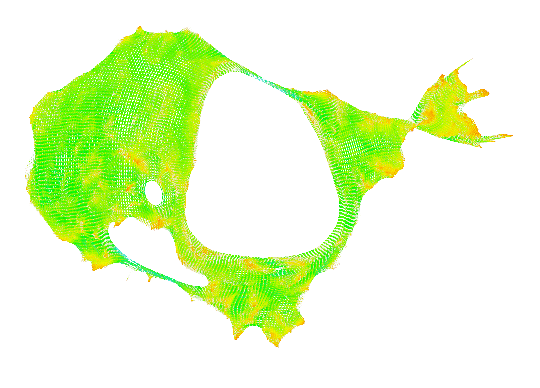
\includegraphics[height=\paperheight, width=\paperwidth]{DIMACS10@fe_ocean.png}}

\begin{frame}
% this frame just has the graph
\blfootnote{DIMACS10@fe\_ocean $143437$ Vertices, $409593$ Edges}
\end{frame}
\usebackgroundtemplate{}

\begin{frame}
\frametitle{fe\_ocean}

\begin{center}
\begin{tikzpicture}
\begin{axis}[
title=fe\_ocean,
width=1\textwidth,
height=0.55\textwidth,
xlabel=Degree,
ylabel=Vertices,
bar width = 20pt,
ybar,
]
\addplot table[x={degree}, y={vertices}, col sep=comma] {feocean.csv};
\end{axis}
\end{tikzpicture}
\end{center}

\begin{itemize}
\item mostly degree 6 vertices
\item low amount of degree 1 and 2 vertices
\end{itemize}	
\end{frame}

\begin{frame}
\frametitle{Heuristic Good Case}
\begin{itemize}
\item Graph we perform well on \\
$\rightarrow$ coAuthorsDBLP
\item Actual VC size:\quad\quad 155618
\item Heuristic VC size:\quad 155620
\end{itemize}
\end{frame}

\begin{frame}
\frametitle{EDIT: Graph Source}
https://www.cise.ufl.edu/research/sparse/matrices/\\
DIMACS10/coAuthorsDBLP.html
\end{frame}

\usebackgroundtemplate{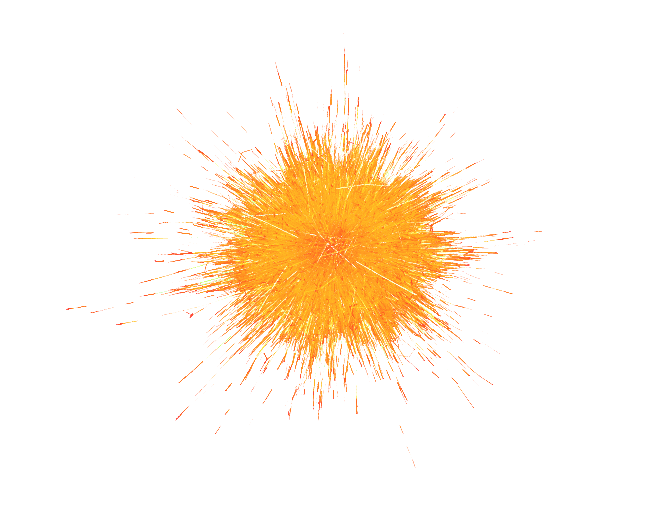
\includegraphics[height=\paperheight, width= \paperwidth]{DIMACS10@coAuthorsDBLP}}

\begin{frame}
\blfootnote{DIMACS10@coAuthorsDBLP $299067$ Vertices, $977676$ Edges}
\end{frame}
\usebackgroundtemplate{}

\begin{frame}
\begin{tikzpicture}
\begin{axis}[
title=coAuthorsDBLP,
width=1\textwidth,
height=0.55\textwidth,
bar width=0.64pt,
xlabel=Degree,
ylabel=Vertices,
ybar,
ymode=log]
\addplot table[x={degree}, y={vertices}, col sep=comma] {coAuthorsDBLP.csv};
\end{axis}
\end{tikzpicture}
\end{frame}
\begin{frame}
\frametitle{Conclusion - Heuristic}

\begin{itemize}
\item missing good heuristics for local structures
\item too cautious with "heavy" reductions
\end{itemize}
\end{frame}

	

	
%	\begin{frame}
%		%TODO some conclusions and an outlook to what we will be doing
%		\frametitle{Outlook on Future Improvements}
%		
%		\begin{itemize}
%			\item[-] 
%			\item[-] 
%			\item[-] 
%			\item[-] 
%		\end{itemize}
%		


		
%	\end{frame}
	\begin{frame}
		\frametitle{Thanks for your attention}
		\centering	\Huge Questions?
	\end{frame}

\end{document}